\chapter{Accepttestspecifikation}
Dette dokument specificerer accepttesten af systemet for Rambøll Tilsyn jf. kravspecifikationen. \\
Accepttesten er blevet kørt som dry run, sammen med vejleder Lars Christian Jensen. Denne blev udført op emulator, der vil dog i brugertesten med Rambøll, skulle bruges en fysisk enhed, i form af f.eks. en iPad.  \\


\section{Login}

\begin{figure}[H] % (alternativt [H])
	\centering
	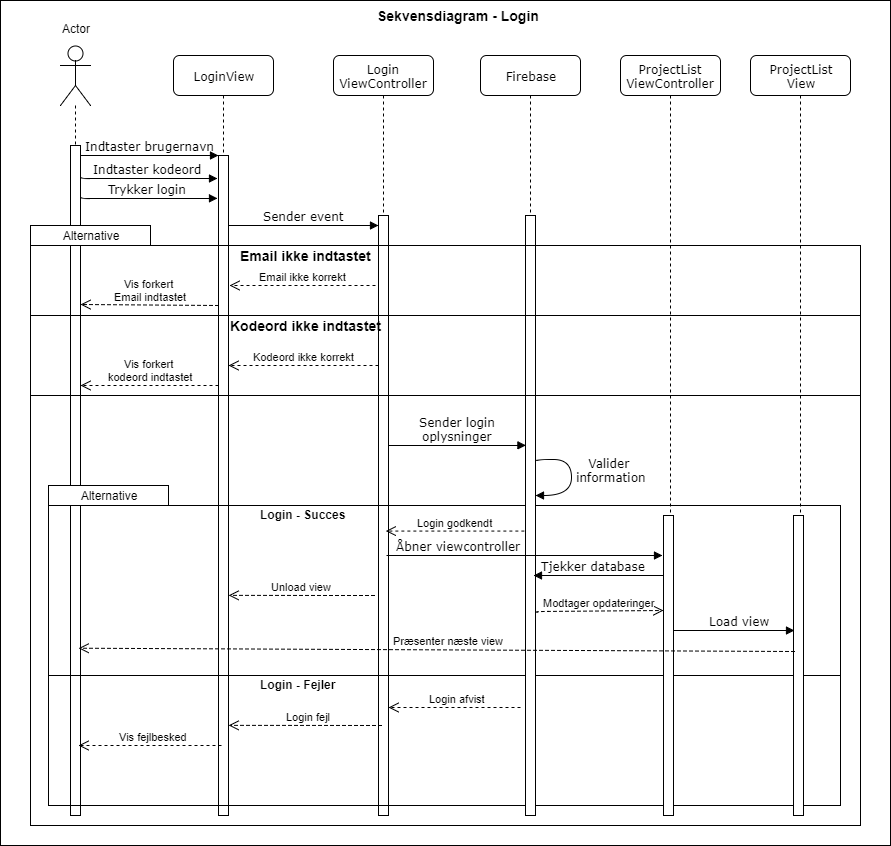
\includegraphics[width=1.1\textwidth]{../ArkitekturDesign/Design/Login/LoginSekvensDiagram}
	\caption{Sekvensdiagram for Login i Rambøll Tilsyn.}
	\label{fig:LoginSekvens}
\end{figure}
\section{Accepttest for Opret bruger (CRS-2)}
Dette afsnit beskriver accepttesten for Opret bruger.

\textbf{User story beskrivelse} \\
Som bruger \\
Ønsker jeg at kunne oprette en bruger på applikationen \\
For at kunne give en anden bruger adgang til systemet

\begin{table}[H]
	\centering
	\begin{tabular}{|ll|l|ll|} \hline
		\textbf{Scenarie} &  & \textbf{Beskrivelse}&  \textbf{Godkendt}&  \\ \hline
		Opret bruger&  &  Når alt information omkring en bruger &  OK&  \\
		& & er udfyldt, og der trykkes opret bruger, bliver brugeren oprettet& & \\ \hline
	\end{tabular}
	\caption{Accepttest for Opret bruger (CRS-2)}
	\label{AcceptOpretBruger}
\end{table}

\clearpage
\section{Accepttest for Rediger brugeroplysninger (CRS-3)}
Dette afsnit beskriver accepttesten for Rediger brugeroplysninger.

\textbf{User story beskrivelse} \\
Som bruger\\
Ønsker jeg at kunne ændre brugeroplysninger \\
For at have aktuelle oplysninger

\begin{table}[H]
	\centering
	\begin{tabular}{|ll|l|ll|} \hline
		\textbf{Scenarie} &  & \textbf{Beskrivelse}&  \textbf{Godkendt}&  \\ \hline
		Rediger kode&  &  Når bruger har ændret sit kodeord &  Ikke OK&  \\
		& & og trykker på gem, er kodeordet ændret& & \\ \hline
		Rediger for- og efternavn&  &  Når bruger har ændret enten fornavn eller efternavn &  Ikke OK&  \\
		& & eller begge dele og trykker på gem, er navne-ændringerne & & \\
		& & ændret& & \\ \hline
		Rediger telefonnummer&  &  Når bruger har ændret sit telefonnummer &  Ikke OK&  \\
		& & og trykker på gem, er telefonnummeret ændret& & \\ \hline
	\end{tabular}
	\caption{Accepttest for Rediger brugeroplysninger (CRS-3)}
	\label{AcceptRedigerBruger}
\end{table}
\section{Accepttest for Opret en registrering på PDF-tegning (CRS-4)}
Dette afsnit beskriver accepttesten for Opret en registrering på PDF-tegning.

\textbf{User story beskrivelse} \\
Som bruger \\
Ønsker jeg at kunne oprette en registrering på en PDF \\
For kunne lave en registrering på et givent projekts PDF-tegning

\begin{table}[H]
	\centering
	\begin{tabular}{|ll|l|ll|} \hline
		\textbf{Scenarie} &  & \textbf{Beskrivelse}&  \textbf{Godkendt}&  \\ \hline
		Opret en registrering på PDF-tegning&  &  Når bruger vælger et projekt &  OK&  \\
		& & kan der oprettes en registrering& & \\ 
			& & på en PDF-tegning& & \\ \hline
	\end{tabular}
	\caption{Accepttest for Opret en registrering på PDF tegning (CRS-4)}
	\label{AcceptPDF}
\end{table}

\clearpage
\section{Accepttest for Opret fluebens objekt på PDF tegning (CRS-5)}
Dette afsnit beskriver accepttesten for Opret fluebens objekt på PDF tegning.

\textbf{User story beskrivelse} \\
Som bruger \\
Ønsker jeg at kunne oprette et fluebens objekt på en PDF tegning \\
For at kunne opdatere min registrering på et givent projekt

\begin{table}[H]
	\centering
	\begin{tabular}{|ll|l|ll|} \hline
		\textbf{Scenarie} &  & \textbf{Beskrivelse}&  \textbf{Godkendt}&  \\ \hline
		Opret fluebens objekt på PDF tegning&  &  Når bruger er inde i en registrering &  OK&  \\
		& & er det mulighed at oprette et fluebens objekt& & \\ 
		& & på PDF tegning& & \\ \hline
	\end{tabular}
	\caption{Accepttest for Opret fluebens objekt på PDF tegning (CRS-5)}
	\label{AcceptFlueben}
\end{table}
\section{Accepttest for Opret billedeobjekt på PDF-tegning (CRS-6)}
Dette afsnit beskriver accepttesten for Opret billedeobjekt på PDF-tegning.

\textbf{User story beskrivelse} \\
Som bruger \\
Ønsker jeg at kunne oprette et billedeobjekt på en PDF-tegning \\
For at kunne opdatere min registrering på et givent projekt

\begin{table}[H]
	\centering
	\begin{tabular}{|ll|l|ll|} \hline
		\textbf{Scenarie} &  & \textbf{Beskrivelse}&  \textbf{Godkendt}&  \\ \hline
		Opret billede objekt på PDF-tegning&  &  Når bruger er inde i en registrering &  Ikke OK&  \\
		& & er det mulighed at oprette et billedeobjekt& & \\ 
		& & på PDF-tegning& & \\ \hline
	\end{tabular}
	\caption{Accepttest for Opret billedeobjekt på PDF-tegning (CRS-6)}
	\label{AcceptBillede}
\end{table}

\clearpage
\section{Accepttest for Opret tekstfeltobjekt på PDF-tegning (CRS-7)}
Dette afsnit beskriver accepttesten for Opret tekstfeltobjekt på PDF-tegning.

\textbf{User story beskrivelse} \\
Som bruger \\
Ønsker jeg at kunne oprette et tekstfeltobjekt på en PDF \\
For at kunne opdatere min registrering på et givent projekt

\begin{table}[H]
	\centering
	\begin{tabular}{|ll|l|ll|} \hline
		\textbf{Scenarie} &  & \textbf{Beskrivelse}&  \textbf{Godkendt}&  \\ \hline
		Opret tekstfeltobjekt på PDF-tegning&  &  Når bruger er inde i en registrering &  Ikke OK&  \\
		& & er det mulighed at oprette et tekstfeltsobjekt& & \\ 
		& & på PDF-tegning& & \\ \hline
	\end{tabular}
	\caption{Accepttest for Opret tekstfeltobjekt på PDF-tegning (CRS-7)}
	\label{AcceptTekstfelt}
\end{table}
\section{Accepttest for Opret kommentarfeltobjekt på PDF-tegning (CRS-8)}
Dette afsnit beskriver accepttesten for Opret kommentarfeltobjekt på PDF-tegning.

\textbf{User story beskrivelse} \\
Som bruger \\
Ønsker jeg at kunne oprette et kommentarfeltobjekt på en PDF \\
For at kunne opdatere min registrering på et givent projekt

\begin{table}[H]
	\centering
	\begin{tabular}{|ll|l|ll|} \hline
		\textbf{Scenarie} &  & \textbf{Beskrivelse}&  \textbf{Godkendt}&  \\ \hline
		Opret kommentarfeltobjekt på PDF-tegning&  &  Når bruger er inde i en registrering &  Ikke OK&  \\
		& & er det mulighed at oprette et kommentarfelt- & & \\ 
		& & objekt på PDF-tegning& & \\ \hline
	\end{tabular}
	\caption{Accepttest for Opret kommentarfeltobjekt på PDF-tegning (CRS-8)}
	\label{AcceptKommentarfelt}
\end{table}

\clearpage
\section{Accepttest for Opret pil objekt på PDF tegning (CRS-9)}
Dette afsnit beskriver accepttesten for Opret pil objekt på PDF tegning.

\textbf{User story beskrivelse} \\
Som bruger \\
Ønsker jeg at kunne oprette et pil objekt på en PDF \\
For at kunne opdatere min registrering på et givent projekt

\begin{table}[H]
	\centering
	\begin{tabular}{|ll|l|ll|} \hline
		\textbf{Scenarie} &  & \textbf{Beskrivelse}&  \textbf{Godkendt}&  \\ \hline
		Opret pil objekt på PDF tegning&  &  Når bruger er inde i en registrering &  Ikke OK&  \\
		& & er det mulighed at oprette et pil objekt& & \\ 
		& & på PDF tegning& & \\ \hline
	\end{tabular}
	\caption{Accepttest for Opret pil objekt på PDF tegning (CRS-9)}
	\label{AcceptPil}
\end{table}
\section{Accepttest for Opret cirkelobjekt på PDF-tegning (CRS-10)}
Dette afsnit beskriver accepttesten for Opret cirkelobjekt på PDF-tegning.

\textbf{User story beskrivelse} \\
Som bruger \\
Ønsker jeg at kunne oprette et cirkelobjekt på en PDF \\
For at kunne opdatere min registrering på et givent projekt

\begin{table}[H]
	\centering
	\begin{tabular}{|ll|l|ll|} \hline
		\textbf{Scenarie} &  & \textbf{Beskrivelse}&  \textbf{Godkendt}&  \\ \hline
		Opret cirkelobjekt på PDF tegning&  &  Når bruger er inde i en registrering &  OK&  \\
		& & er det mulighed at oprette et cirkelobjekt& & \\ 
		& & på PDF-tegning& & \\ \hline
	\end{tabular}
	\caption{Accepttest for Opret cirkelobjekt på PDF-tegning (CRS-10)}
	\label{AcceptCirkel}
\end{table}
\section{Accepttest for Opret minusobjekt på PDF-tegning (CRS-11)}
Dette afsnit beskriver accepttesten for Opret minusobjekt på PDF-tegning.

\textbf{User story beskrivelse} \\
Som bruger \\
Ønsker jeg at kunne oprette et minusobjekt på en PDF \\
For at kunne opdatere min registrering på et givent projekt

\begin{table}[H]
	\centering
	\begin{tabular}{|ll|l|ll|} \hline
		\textbf{Scenarie} &  & \textbf{Beskrivelse}&  \textbf{Godkendt}&  \\ \hline
		Opret minusobjekt på PDF-tegning&  &  Når bruger er inde i en registrering &  OK&  \\
		& & kan der oprettes et minusobjekt& & \\ 
		& & på PDF-tegning& & \\ \hline
	\end{tabular}
	\caption{Accepttest for Opret minusobjekt på PDF-tegning (CRS-11)}
	\label{AcceptMinus}
\end{table}

\clearpage
\section{Accepttest for Slet objekt på PDF tegning (CRS-12)}
Dette afsnit beskriver accepttesten for Slet objekt på PDF tegning.

\textbf{User story beskrivelse} \\
Som bruger \\
Ønsker jeg at kunne slette et objekt på en PDF \\
For at kunne opdatere min registrering på et givent projekt

\begin{table}[H]
	\centering
	\begin{tabular}{|ll|l|ll|} \hline
		\textbf{Scenarie} &  & \textbf{Beskrivelse}&  \textbf{Godkendt}&  \\ \hline
		Slet objekt på PDF tegning&  &  Når bruger er inde i en registrering &  Ikke OK&  \\
		& & er det mulighed at slette et objekt& & \\ 
		& & på PDF tegning& & \\ \hline
	\end{tabular}
	\caption{Accepttest for Slet objekt på PDF tegning (CRS-12)}
	\label{AcceptSlet}
\end{table}
\section{Accepttest for Afslut registrering på PDF tegning (CRS-13)}
Dette afsnit beskriver accepttesten for Afslut registrering på PDF tegning.

\textbf{User story beskrivelse} \\
Som bruger \\
Ønsker jeg at kunne afslutte min registrering \\
For at kunne afslutte en registrering på et projekt

\begin{table}[H]
	\centering
	\begin{tabular}{|ll|l|ll|} \hline
		\textbf{Scenarie} &  & \textbf{Beskrivelse}&  \textbf{Godkendt}&  \\ \hline
		Afslut registrering på PDF tegning&  &  Når bruger er færdig med sin &  Ikke OK&  \\
		& & registrering er der mulighed for at& & \\
		& & at afslutte denne& & \\ \hline
	\end{tabular}
	\caption{Accepttest for Afslut registrering på PDF tegning (CRS-13)}
	\label{AcceptAfslutPDF}
\end{table}
\section{Accepttest for Opret en registrering uden PDF tegning (CRS-14)}
Dette afsnit beskriver accepttesten for Opret en registrering uden PDF tegning.

\textbf{User story beskrivelse} \\
Som bruger \\
Ønsker jeg at kunne oprette en registrering uden en PDF  \\
For kunne lave en registrering på et givent projekt

\begin{table}[H]
	\centering
	\begin{tabular}{|ll|l|ll|} \hline
		\textbf{Scenarie} &  & \textbf{Beskrivelse}&  \textbf{Godkendt}&  \\ \hline
		Opret en registrering uden PDF tegning&  &  Når bruger vælger et projekt &  Ikke OK&  \\
		& & er der mulighed for at lave en registrering& & \\ 
			& & uden en PDF tegning& & \\ \hline
	\end{tabular}
	\caption{Accepttest for Opret en registrering uden PDF tegning (CRS-14)}
	\label{AcceptUdenPDF}
\end{table}

\clearpage
\section{Accepttest for Afslut registrering uden PDF tegning (CRS-15)}
Dette afsnit beskriver accepttesten for Afslut registrering på PDF tegning.

\textbf{User story beskrivelse} \\
Som bruger \\
Ønsker jeg at kunne afslutte min registrering \\
For at kunne afslutte en registrering på et projekt

\begin{table}[H]
	\centering
	\begin{tabular}{|ll|l|ll|} \hline
		\textbf{Scenarie} &  & \textbf{Beskrivelse}&  \textbf{Godkendt}&  \\ \hline
		Afslut registrering uden PDF tegning&  &  Når bruger er færdig med sin &  Ikke OK&  \\
		& & registrering er der mulighed for at& & \\
		& & afslutte denne& & \\ \hline
	\end{tabular}
	\caption{Accepttest for Afslut registrering uden PDF tegning (CRS-15)}
	\label{AcceptAfslutUdenPDF}
\end{table}
\section{Accepttest for Opret projekt (CRS-16)}
Dette afsnit beskriver accepttesten for Opret projekt.

\textbf{User story beskrivelse} \\
Som bruger \\
Ønsker jeg at kunne oprette projektoplysninger \\
For at have aktuelle oplysninger om projektet

\begin{table}[H]
	\centering
	\begin{tabular}{|ll|l|ll|} \hline
		\textbf{Scenarie} &  & \textbf{Beskrivelse}&  \textbf{Godkendt}&  \\ \hline
		Opret projekt&  &  Når alt information omkring et projekt &  Ikke OK&  \\
		& & er udfyldt, og der trykkes opret projekt, bliver brugeren oprettet& & \\ \hline
	\end{tabular}
	\caption{Accepttest for Opret projekt (CRS-16)}
	\label{AcceptOpretProjekt}
\end{table}
\section{Accepttest for Rediger projektoplysninger (CRS-17)}
Dette afsnit beskriver accepttesten for Rediger brugeroplysninger.

\textbf{User story beskrivelse} \\
Som bruger \\
Ønsker jeg at kunne ændre projektoplysninger \\
For at have aktuelle oplysninger

\begin{table}[H]
	\centering
	\begin{tabular}{|ll|l|ll|} \hline
		\textbf{Scenarie} &  & \textbf{Beskrivelse}&  \textbf{Godkendt}&  \\ \hline
		Rediger projekt navn&  &  Når bruger har ændret sit projekt navn &  Ikke OK&  \\
		& & og trykker på gem, er projekt navnet ændret& & \\ \hline
		Rediger projekt nummer&  &  Når bruger har ændret projekt nummer &  Ikke OK&  \\
		& & og trykker på gem, er projekt nummeret ændret & & \\ \hline
		Rediger projekt adresse&  &  Når bruger har ændret projekt adresse &  Ikke OK&  \\
		& & og trykker på gem, er projekt adresse ændret& & \\ \hline
		Rediger entreprenør information&  &  Når bruger har ændret alle entreprenør &  Ikke OK&  \\
		& & informationer og trykker på gem, er entreprenør& & \\
		& & informationerne ændret& & \\ \hline
	\end{tabular}
	\caption{Accepttest for Rediger projektoplysninger (CRS-17)}
	\label{AcceptRedigerProjekt}
\end{table}

\clearpage
\section{Accepttest for Se tilsynsrapporter (CRS-18)}
Dette afsnit beskriver accepttesten for Afslut registrering på PDF tegning.

\textbf{User story beskrivelse} \\
Som bruger \\
Ønsker jeg at kunne se tilsynsrapporter for et givent projekt \\
For at kunne følge byggeriets gang

\begin{table}[H]
	\centering
	\begin{tabular}{|ll|l|ll|} \hline
		\textbf{Scenarie} &  & \textbf{Beskrivelse}&  \textbf{Godkendt}&  \\ \hline
		Se tilsynsrapporter&  &  Bruger vil gerne have mulighed for &  Ikke OK&  \\
		& & at få en liste over registreringer & & \\
		& & fordi forskellige projekter& & \\ \hline
	\end{tabular}
	\caption{Accepttest for Se tilsynsrapporter (CRS-18)}
	\label{AcceptTilsyn}
\end{table}
\section{Accepttest for Opret subprojekt (CRS-19)}
Dette afsnit beskriver accepttesten for Opret sub projekt.

\textbf{User story beskrivelse} \\
Som bruger \\
Ønsker jeg at kunne opdele et projekt i flere projekter \\
For at have give et beder overblik over projektet

\begin{table}[H]
	\centering
	\begin{tabular}{|ll|l|ll|} \hline
		\textbf{Scenarie} &  & \textbf{Beskrivelse}&  \textbf{Godkendt}&  \\ \hline
		Opret sub projekt&  &  Når et projekt oprettes er der &  Ikke OK&  \\
		& & mulighed for at oprette sub projekter & & \\
		& & for at opdele et stort projekt i mindre projekter& & \\ \hline
	\end{tabular}
	\caption{Accepttest for Opret subprojekt (CRS-19)}
	\label{AcceptSubProjekt}
\end{table}
